\tutorial{1}{Getting started}

\begin{goal}
You install the Raven--MODFLOW~6 package, check that Raven finds the MODFLOW~6 library, run the Liard River example (Raven
builds a groundwater model under three subbasins and runs it with Raven every day), and read and plot its groundwater
results: the budget (\cmd{GWBudget.csv}), the water table under each HRU (\cmd{GWHRUState.csv}) and the head field of
MODFLOW. Time: about 20 minutes.
\end{goal}

\section{What you need}
\begin{itemize}
\item A Linux computer (x86\_64) with a terminal. The package holds a ready-to-run Raven built with the MODFLOW~6 library.
      \emph{Windows users:} install the Windows Subsystem for Linux (WSL, \cmd{wsl --install} in PowerShell, then Ubuntu)
      and follow the tutorials in its terminal; your Windows files are under \cmd{/mnt/c/}.
\item Python~3 with numpy, pandas and matplotlib (\cmd{python3 -m pip install numpy pandas matplotlib}). Tutorial~5 also uses
      FloPy for particle tracking (\cmd{python3 -m pip install flopy}).
\item Two zip files: the release package \cmd{Raven\_MF6\_package.zip} and the tutorial files
      \cmd{Raven\_MF6\_Tutorial\_Files.zip}, both from the same release: the tutorials show the numbers and tools of the
      package they come with. Tutorial~6 also needs OSTRICH (it tells you where to get it).
\end{itemize}
All commands are typed in a terminal. Lines starting with \cmd{\$} are what you type; the lines below them are what the
computer answers (long answers are shortened with \cmd{...}). The examples show a user called \cmd{user}, whose home
folder is \cmd{/home/user}; yours will show your own name.

\section{Install the package and the tutorial files}
Put both zip files in your home folder and unpack them:
\begin{shell}
$ cd ~
$ unzip -q Raven_MF6_package.zip
$ unzip -q Raven_MF6_Tutorial_Files.zip
\end{shell}
\cmd{unzip -q} answers nothing. You now have \cmd{\textasciitilde/Raven\_MF6\_linux} (the package) and
\cmd{\textasciitilde/Raven\_MF6\_Tutorials} (one folder per tutorial, each with a \cmd{start} and a \cmd{finished} state, and the
\cmd{scripts} the tutorials use). Give them short names for this terminal; every tutorial uses these four variables:
\begin{shell}
$ export PKG=~/Raven_MF6_linux
$ export RAVEN=$PKG/bin/Raven
$ export TUT=~/Raven_MF6_Tutorials
$ export TOOLS=$PKG/raven-mf6-extra/tools
\end{shell}
\begin{note}[Every new terminal]
\cmd{export} lasts for this terminal only. Add the four lines to the end of \cmd{\textasciitilde/.bashrc} to have them in every
new terminal, or type them again.
\end{note}
Look at what the package holds:
\term{t1_ls_pkg.txt}
\cmd{bin/Raven} is Raven with the coupling, \cmd{bin/libmf6.so} the MODFLOW~6 library (version \V{t1:mf6ver}). Raven finds the
library beside itself; nothing else needs to be set. The manual is \cmd{Raven\_MF6\_Manual.pdf}.

\subsection{Check the version}
The tutorials were made with the package built from commit \cmd{\V{t1:reqcode}} of the Raven code and commit
\cmd{\V{t1:reqextra}} of its extra tools (\cmd{raven-mf6-extra}). The package names its commits in
\cmd{source/COMMITS.txt}:
\begin{shell}
$ cut -c1-90 $PKG/source/COMMITS.txt
\end{shell}
The first line must name commit \cmd{\V{t1:reqcode}...} (or a later one), the second \cmd{\V{t1:reqextra}...} (or a later
one). An older package runs the tutorials too, but some of its numbers differ from those printed here and some of its tools
are missing; use the package that came with these tutorial files.

\subsection{Check the installation}
The package's \cmd{README.md} gives the check: it unpacks one small script from the source archive and runs \cmd{bin/Raven}
on a tiny coupled model.
\begin{shell}
$ cd $PKG
$ tar xzf source/raven_code_src.tar.gz raven-soil-zone/cmake/RavenMF6InstallCheck.py
\end{shell}
\term{t1_installcheck.txt}
\begin{tocheck}
The last line must read \cmd{install check: PASS}, and the line \emph{the library beside Raven was used} must name
\cmd{\$PKG/bin/libmf6.so} with version \V{t1:mf6ver}.
\end{tocheck}
\begin{trouble}
\begin{itemize}
\item \cmd{Permission denied} for \cmd{bin/Raven}: the unzip program lost the execute permission; type
      \cmd{chmod +x \$PKG/bin/Raven}.
\item \cmd{cannot load MODFLOW 6 library}: \cmd{libmf6.so} is not beside \cmd{Raven}; keep the two files together in \cmd{bin/}.
\item \cmd{install check: FAIL} on another line: the line marked \cmd{FAIL} says what is missing. On Linux other than x86\_64 the
      package's programs do not run: build Raven from the source archive (\cmd{README.md}, ``Build from source'').
\end{itemize}
\end{trouble}

\subsection{Unpack the tools and the user guide}
The tools used in the tutorials (\cmd{plot\_soilzone.py}, \cmd{make\_prt.py}), the user guide and the test suite are in the
second source archive. Unpack it inside the package:
\begin{shell}
$ cd $PKG
$ tar xzf source/raven_extra_docs_tests.tar.gz
\end{shell}
\term{t1_ls_tools.txt}
The user guide is \cmd{\$PKG/raven-mf6-extra/docs/Raven\_MF6\_Groundwater\_UserGuide.md}.

\section{Run the Liard River example}
The package's \cmd{examples/Liard\_groundwater} is the Liard River Raven model (65 subbasins in northern British Columbia
and Yukon) with a hypothetical aquifer under three subbasins. Raven builds the MODFLOW~6 model itself, from HRU polygons,
river lines, a land-surface raster (DEM) and a bedrock raster. Work on a copy, so that the package stays as it came:
\begin{shell}
$ mkdir -p ~/work
$ cp -r $PKG/examples ~/work/
$ cd ~/work/examples/Liard_groundwater
\end{shell}
The example simulates \V{t1:fullDays} days (\V{t1:fullYears} years, about \V{t1:fullmin}~minutes). For a first run shorten it to one year: the
\cmd{:Duration} line of \cmd{Liard.rvi} holds the number of days. Change it with a text editor, or with \cmd{sed}:
\begin{shell}
$ sed -i 's/^:Duration           7305 /:Duration           365 /' Liard.rvi
\end{shell}
\term{t1_duration.txt}
Now run Raven. \cmd{Liard} is the model name (Raven reads \cmd{Liard.rvi}, \cmd{.rvh}, \cmd{.rvp}, \cmd{.rvt},
\cmd{.rvc} and, for groundwater, \cmd{Liard.rvg}); \cmd{-o out/} is the output folder.
\term{t1_run.txt}
Raven prints its progress (shortened here). The run takes about \V{t1:runsec}~seconds.
\begin{tocheck}
The last line must be \cmd{Exiting Gracefully: Successful Simulation}, and Raven reports that the groundwater model was
initialised. Warnings are listed in \cmd{out/Raven\_errors.txt}; for this example they say that the stand-in HRU polygons
do not match the \cmd{.rvh} areas (the example's \cmd{README.md} explains why; water volumes are still exchanged exactly).
\end{tocheck}
\begin{trouble}
\begin{itemize}
\item \cmd{\$RAVEN: command not found} or an empty variable: type the \cmd{export} lines of Section~1 again in this terminal.
\item \cmd{Cannot find or read .rvh file} (or another file): you are not in the example folder; \cmd{cd} there first.
\item Any other stop: the reason is in \cmd{out/Raven\_errors.txt}, and the user guide's ``Troubleshooting'' table lists the
      messages of the groundwater coupling.
\end{itemize}
\end{trouble}

\section{The results}
\term{t1_ls_out.txt}
Besides Raven's usual outputs (\cmd{Hydrographs.csv}, \cmd{Diagnostics.csv}, \cmd{WatershedStorage.csv}, \cmd{solution.rvc}) a
coupled run writes the groundwater files \cmd{GWModelSummary.txt}, \cmd{GWBudget.csv}, \cmd{GWHRUState.csv} and
\cmd{GWConnectivity.csv}, and the MODFLOW~6 model itself in \cmd{out/mf6/} (it can be opened with FloPy or ModelMuse).

\subsection{What Raven built: \texttt{GWModelSummary.txt}}
\term{t1_summary.txt}
Raven laid a regular grid of \V{t1:nlay}~layers, \V{t1:nrow}~rows and \V{t1:ncol}~columns of \V{t1:cell}~m cells over the
\V{t1:nhru} coupled HRUs, kept the \V{t1:activecols} columns that lie under them, and placed \V{t1:rivcells} river cells
along the river lines. The second part of the file (not shown) lists every coupled HRU with its area in the \cmd{.rvh}, the
area of its polygon and the number of cells it covers.

\subsection{The groundwater budget: \texttt{GWBudget.csv}}
One line per day, with \V{t1:ncolsBudget} columns. The first ones:
\term{t1_budget_head.txt}
All flows are in m\textsuperscript{3}/d over the whole groundwater model. The most important columns:
\begin{center}\small
\begin{tabularx}{\linewidth}{>{\raggedright\arraybackslash}p{0.33\linewidth}X}\toprule
Column & Meaning (mean of this run)\\\midrule
\cmd{Raven recharge}, \cmd{MF6 recharge} & water Raven's processes put into \cmd{GROUNDWATER} and what MODFLOW received
  (equal) (\V{t1:rech} million m\textsuperscript{3}/d)\\
\cmd{seepage to Raven} & groundwater seeping out where the water table reaches the model top; it returns to Raven's lowest soil
  layer (\V{t1:seep} million m\textsuperscript{3}/d)\\
\cmd{storage release} & water released from aquifer storage (positive: the aquifer drains) (\V{t1:stor} million m\textsuperscript{3}/d)\\
\cmd{MF6 balance error} & MODFLOW's own balance error, in m\textsuperscript{3}/d and \% (largest: \V{t1:balerr}~\%)\\
\cmd{outer iterations}, \cmd{converged} & how hard MODFLOW worked (at most \V{t1:maxouter} iterations) and whether it
  converged (1)\\
\cmd{river leakage to aquifer}, \cmd{aquifer discharge to rivers} & exchange with the river cells
  (\V{t1:fromriv} and \V{t1:toriv} million m\textsuperscript{3}/d), taken from or added to Raven's reaches\\\bottomrule
\end{tabularx}\end{center}
The user guide (section~5) lists every column; wells, head boundaries, water-table evaporation, surface stores,
reservoirs and the soil zone have columns of their own (zero here).

\subsection{The water table: \texttt{GWHRUState.csv}}
\term{t1_hrustate_head.txt}
For every coupled HRU, the mean head (\cmd{head\_ID}) and the mean depth of the water table below the land surface
(\cmd{wtdepth\_ID}) of the cells under it. In this run the mean depths range from \V{t1:wtmin}~m to \V{t1:wtmax}~m.

\subsection{Check the water balance}
\cmd{tools\_audit.py}, shipped with the example, checks every balance identity of a run:
\term{t1_audit.txt}
\begin{tocheck}
\begin{itemize}
\item \cmd{recharge: (Raven - MF6 - dStore - toCHD)/Raven} is 0: every cubic metre of recharge reached MODFLOW;
\item \cmd{MF6 cumulative residual / gross flow} is tiny (here \V{t1:auditRes});
\item \cmd{unconverged steps} is \V{t1:auditUnconv}, \cmd{ERROR lines} 0, and the river bookkeeping is at round-off;
\item \cmd{Raven MB error max [mm]} is Raven's own water-balance error (\V{t1:auditMB}~mm here).
\end{itemize}
\end{tocheck}

\subsection{Plot the results}
The tutorial files contain a plotting script (it needs numpy, pandas and matplotlib, not FloPy):
\term{t1_plot.txt}
It writes four pictures into \cmd{out/} (three here: the Liard example has no observation wells) and prints a summary.
Figures~\ref{fig:t1budget} to~\ref{fig:t1map} are those pictures.
\begin{figure}[!htbp]\centering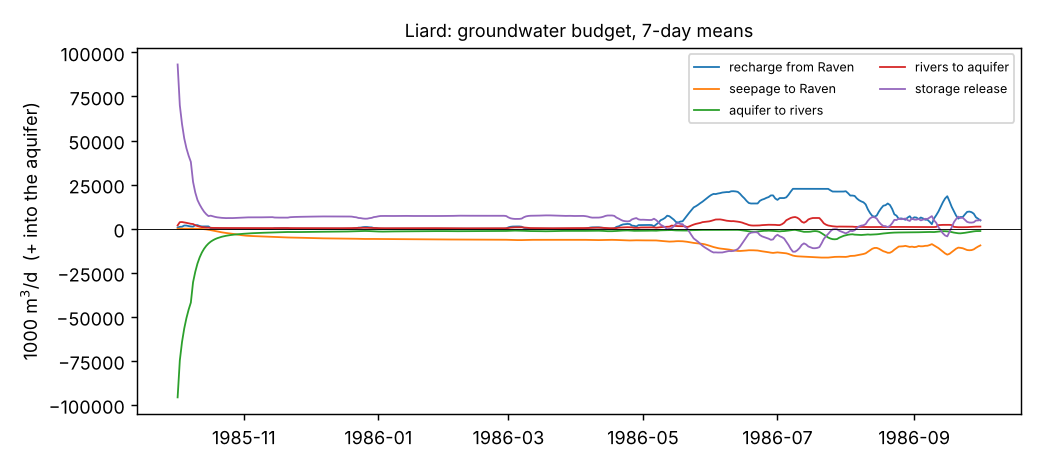
\includegraphics[width=0.9\linewidth]{figures/t1_gw_budget.png}
\caption{\cmd{gw\_budget.png}: the daily groundwater budget of the Liard example (7-day means; positive: into the
aquifer). The large flows of the first weeks are the aquifer adjusting from its initial heads (\cmd{INITIAL\_HEAD\_DEPTH}
of the profiles); afterwards seepage and discharge to the rivers return the recharge, and storage takes up the difference.}\label{fig:t1budget}\end{figure}
\begin{figure}[!htbp]\centering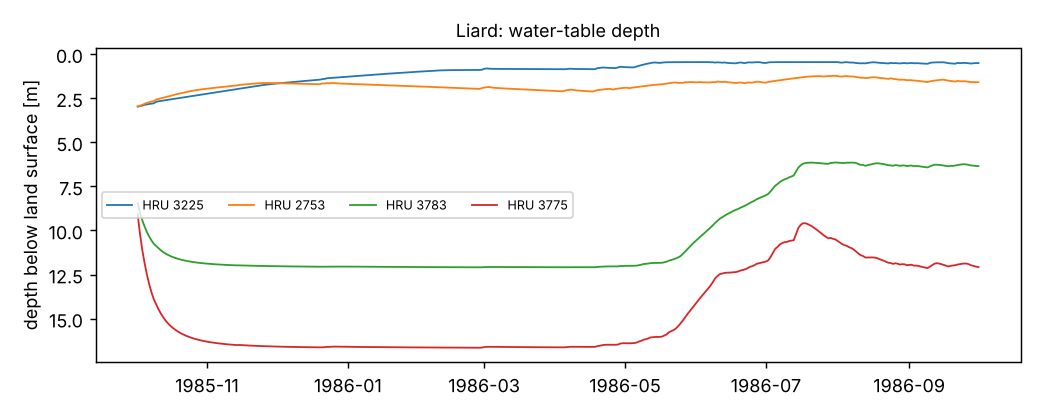
\includegraphics[width=0.9\linewidth]{figures/t1_gw_watertable.png}
\caption{\cmd{gw\_watertable.png}: water-table depth under the two shallowest and the two deepest HRUs
(\cmd{--hrus ID ...} chooses others).}\label{fig:t1wt}\end{figure}
\begin{figure}[!htbp]\centering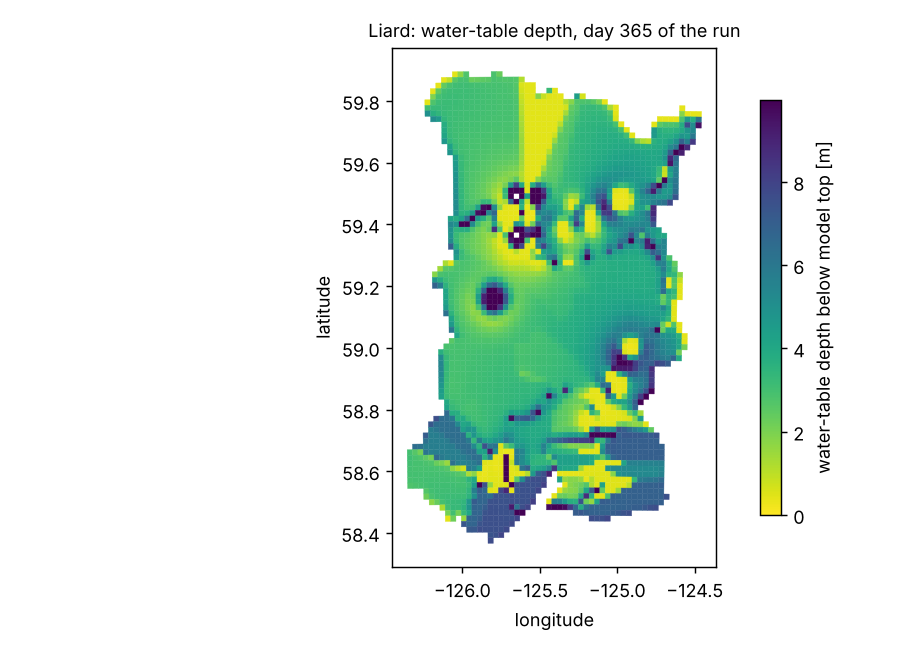
\includegraphics[width=0.72\linewidth]{figures/t1_gw_map.png}
\caption{\cmd{gw\_map.png}: water-table depth in every active column at the last saved head field of \cmd{out/mf6/gwf.hds}
(\cmd{:HeadSaveFrequency} in \cmd{Liard.rvg} sets how often MODFLOW saves it), on the cells of
\cmd{out/mf6/grid\_cells.geojson}.}\label{fig:t1map}\end{figure}
\begin{note}[Reading MODFLOW's files yourself]
\cmd{out/mf6/gwf.hds} is a standard MODFLOW~6 head file and \cmd{gwf.dis.grb} its grid; with FloPy,
\cmd{flopy.utils.HeadFile('out/mf6/gwf.hds').get\_data()} returns the last head field. \cmd{grid\_cells.geojson} (all cells in
longitude/latitude, with their number and an \cmd{active} flag) opens in any GIS.
\end{note}

\section{The full run}
Put the \V{t1:fullYears}-year duration back and run again (about \V{t1:fullmin}~minutes on the computer that made this tutorial):
\term{t1_restore.txt}
\begin{shell}
$ $RAVEN Liard -o out/
\end{shell}
Raven ends with \cmd{Exiting Gracefully: Successful Simulation} as before; then audit the run:
\term{t1_audit_full.txt}
\begin{tocheck}
Over \V{t1:fullYears} years: \V{t1:fullUnconv} unconverged steps, a cumulative MODFLOW residual of \V{t1:fullRes} of the gross flow, and
streamflow at the gauges 10BE004, 10BE005 and 10BE010 with Nash--Sutcliffe efficiencies (\cmd{Diagnostics.csv}) of
\V{t1:fullNSE10BE004}, \V{t1:fullNSE10BE005} and \V{t1:fullNSE10BE010}.
\end{tocheck}

\section{What next}
Tutorial~2 builds a groundwater model for a Raven model of your own, from scratch. The example's own \cmd{README.md} and
the manual's chapter ``Applying the coupling'' describe how the Liard example was set up.
